% ! TEX root = ../m3-19-20.tex

\chapter{Spații de probabilitate}

\section{Noțiuni teoretice}

\indent\indent Trecem acum la studiul probabilităților într-un context mai abstract
decît în liceu, unde se defineau și studiau evenimentele aleatoare concret.

\begin{definition}\label{def:spatiu-discret-prob}
  Se numește \emph{spațiu (cîmp) discret de probabilitate} o mulțime finită sau numărabilă
  $ \Omega = (\omega_n)_n $, împreună cu un șir $ (p_n)_n $, cu $ 0 \leq p_n \leq 1 $,
  care satisface condiția $ \ds\sum_n p_n = 1 $.

  Orice submulțime $ A \seq \Omega $ este un \emph{eveniment}, căruia i se atașează
  o probabilitate
  \[
    P(A) = \ds\sum_{\omega_n \in A} p_n.
  \]
\end{definition}

Intuitiv, putem privi elementele mulțimii $ \Omega $ drept \emph{experiențe}, pe
care le putem colecta în \emph{evenimente}, iar $ p_n $ este probabilitatea ca o
experiență să se realizeze.

Alte definiții elementare sînt următoarele:

\begin{definition}\label{def:evenimente}
  \emph{Evenimentul sigur} este un eveniment care se realizează cu certitudine la
  fiecare repetare a experienței.

  \emph{Evenimentul imposibil} nu se produce la nicio efectuare a experienței.

  Dat un eveniment $ A \seq \Omega $, lui i se asociază \emph{evenimentul contrar},
  notat $ \overline{A}, CA $ sau $ A^c $, care constă în nerealizarea lui $ A $.

  Două evenimente $ A, B \seq \Omega $ se numesc \emph{compatibile} dacă se
  pot produce simultan și \emph{incompatibile} în caz contrar.
\end{definition}

Pentru evenimente incompatibile, avem o definiție alternativă, calculatorie:

\begin{definition}\label{def:ev-compat}
  Dacă $ A $ și $ B $ sînt evenimente incompatibile, atunci:
  \[
    P(A \cup B) = P(A) + P(B).
  \]

  Mai general, pentru orice șir $ (A_n) $ de evenimente două cîte două incompatibile,
  avem:
  \[
    P \Big( \bigcup_{n \in \NN} A_n \Big) = \sum_{n \in \NN} P(A_n).
  \]
\end{definition}

Definiția abstractă a contextului în care vom studia teoria probabilităților urmează.

\begin{definition}\label{def:spatiu-prob}
  Se numește \emph{spațiu de probabilitate} un triplet $ (\Omega, \kal{K}, P) $, unde
  $ \Omega $ este o mulțime de evenimente elementare (individuale), $ \kal{K} $ este o
  submulțime a $ \kal{P}(\Omega) $, iar $ P : \kal{K} \to [0, 1] $ este o funcție de
  probabilitate, care satisface:
  \begin{itemize}
  \item $ P(\Omega) = 1 $;
  \item $ P \Big( \ds\bigcup_{n \geq 0} A_n \Big) = \ds\sum_{n \geq 0} P(A_n) $,
    pentru orice șir $ (A_n) $ de evenimente două cîte două incompatibile.
  \end{itemize}
\end{definition}

Pornind de la această definiție generală, putem obține cazuri particulare cunoscute:

\textbf{Definiția clasică a probabilității:} Dacă $ \Omega $ este o mulțime cu $ N $
elemente, putem defini un spațiu discret de probabilitate, definind $ p_n = \frac{1}{N} $,
pentru orice $ n \in \{ 1, \dots, N \}$. În acest caz, probabilitățile sînt egale pentru
toate evenimentele, deci spunem că \emph{evenimentele sînt echiprobabile}. Pentru orice
eveniment $ A \seq \Omega $, avem:
\[
  P(A) = \frac{\mathrm{card}(A)}{\mathrm{card}(\Omega)},
\]
care coincide cu definiția clasică a raportului dintre numărul cazurilor favorabile
unui eveniment și numărul cazurilor posibile.

\vspace{0.3cm}

\textbf{Probabilități geometrice:} Dacă luăm $ \Omega \seq \RR^n $ o submulțime oarecare,
pe care considerăm \emph{măsura Lebesgue} (cea cu ajutorul căreia calculăm integralele),
atunci obținem un spațiu de probabilitate definind pentru orice eveniment $ A $
probabilitatea prin:
\[
  P(A) = \frac{\mu(A)}{\mu(\Omega)},
\]
unde $ \mu $ este măsura Lebesgue din $ \RR^n $ (în particular, e vorba de lungimea $ dl $
pe $ \RR $, aria $ dA = dxdy $ din $ \RR^2 $ etc.).

\vspace{0.3cm}

Următoarele sînt proprietăți elementare ale probabilităților:

Fie $ (\Omega, \kal{K}, P) $ un spațiu de probabilitate.
\begin{enumerate}[(1)]
\item Dacă $ A, B \in \kal{K} $ și $ A \seq B $, atunci $ P(B - A) = P(B) - P(A) $;
\item \textbf{Poincar\'{e}}: Fie $ n $ evenimente arbitrare $ A_1, \dots, A_n \in \kal{K} $.
  Atunci are loc:
  \[
    P \Big( \bigcup_{i = 1}^n A_i \Big) = \sum_{i = 1}^n P(A_i) - \sum_{i \neq j} P(A_i \cap A_j) + %
    \dots + (-1)^{n-1} P(A_1, \dots, A_n).
  \]
\item Pentru orice șir crescător de evenimente $ A_0 \seq A_1 \seq \dots \seq A_n \seq \dots $,
  avem:
  \[
    P \Big( \bigcup_{n\geq 0} \Big) = \lim_{n \to \infty} P(A_n).
  \]
\end{enumerate}

\begin{definition}\label{def:ev-indep}
  Evenimentele $ A $ și $ B $ se numesc \emph{independente} dacă $ P(A \cap B) = P(A) \cdot P(B) $.

  În general, evenimentele $ A_1, \dots, A_n $ se numesc \emph{independente în ansamblu}
  dacă pentru orice $ m \geq n $ și $ 1 \leq j_1 \leq \dots \leq j_m \leq n $, avem:
  \[
    P(A_{j_1} \cap \dots \cap A_{j_m}) = P(A_{j_1}) \cdots P(A_{j_m}).
  \]
\end{definition}

\begin{remark}\label{rk:indep-ans}
  Dacă avem $ n $ evenimente independente două cîte două (cf.\ primei părți a definiției
  de mai sus), nu rezultă neapărat că sînt evenimente în ansamblul lor (cf.\ părții a
  doua a definiției).
\end{remark}

Un contraexemplu, datorat lui S.\ N.\ Bernstein este următorul. Considerăm un tetraedru
omogen cu fețele colorate alb, negru, roșu, iar a patra, cu toate cele trei culori.
Aruncăm acest corp și notăm cu $ A_i $ probabilitatea ca tetraedrul să se așeze (cu baza)
pe fața cu numărul $ i \in \{ 1, 2, 3, 4 \} $. Aceste evenimente sînt elementare și
$ P(A_i) = \dfrac{1}{4}, \forall i $. Acum fie $ A = A_1 \cup A_2, B = A_1 \cup A_3 $ și
$ C = A_1 \cup A_4 $. Atunci $ P(A) = P(B) = P(C) = \dfrac{1}{2} $, deoarece pentru fiecare
culoare sînt 4 cazuri posibile și 2 favorabile (fața cu culoarea respectivă și fața cu
toate culorile).

În plus, avem:
\[
  P(A \cap B) = P(B \cap C) = P(C \cap A) = \frac{1}{4},
\]
deci evenimentele sînt independente două cîte două.

În plus, avem:
\begin{align*}
  P(A \cap B \cap C) &= P(A_1) = \frac{1}{4} \\
  P(A)P(B)P(C) &= \frac{1}{8},
\end{align*}
deci evenimentele nu sînt independente în ansamblul lor.

\vspace{0.3cm}

Mai avem nevoie de următorul concept:

\begin{definition}\label{def:p-cond}
  Fie $ A $ și $ B $ două evenimente, cu $ P(B) \neq 0 $.

  \emph{Probabilitatea lui $ A $ condiționată de $ B $}, notată $ P(A/B) $ sau
  $ P_B(A) $ se definește prin:
  \[
    P(A/B) = \frac{P(A \cap B)}{P(B)}.
  \]
\end{definition}

De asemenea, în calcule, vom mai folosi:

\textbf{Formula de înmulțire a probabilităților}: Fie $ A_1, \dots A_n $ evenimente.
Atunci are loc:
\[
  P(A_1 \cap \dots \cap A_n) = P(A_1) \cdot P(A_2/A_1) \cdot P(A_3/A_1 \cap A_2) \cdots %
  P(A_n/A_1 \cap \dots \cap A_{n-1}).
\]

\vspace{0.3cm}

\textbf{Formula probabilității totale}: Dacă avem descompunerea evenimentului sigur
$ \Omega $ în reuniunea de $ n $ evenimente incompatibile $ H_1, \dots H_n $, atunci
pentru orice eveniment $ A \in \kal{K} $, are loc:
\[
  P(A) = \sum_{i = 1}^n P(A/H_i) \cdot P(H_i).
\]

\vspace{0.3cm}

\textbf{Formula lui Bayes}: În contextul și cu notațiile de mai sus:
\[
  P(H_j/A) = \frac{P(A/H_j) \cdot P(H_j)}{\sum_{i = 1}^n P(A/H_i) \cdot P(H_i)}.
\]

În particular, pentru două evenimente $ A, B $, avem:
\begin{align*}
  P(A) &= P(A/B) \cdot P(B) + P(A/B^c)\cdot P(B^c) \\
  P(B/A) &= \frac{P(A/B) \cdot P(B)}{P(A/B) \cdot P(B) + P(A/B^c) \cdot P(B^c)}.
\end{align*}

%%%%%%%%%%%%%%%%%%%%%%%%%%%%%%%%%%%%%%%%%%%%%%%%%%%%%%%%%%%%%%%%%%%%%%

\section{Exerciții}

\subsection{Calcul \qq{clasic}}

\indent\indent 1. Într-un spațiu de probabilitate se considerăm evenimentele $ A, B $,
cu:
\[
  P(A) = \frac{1}{3}, P(B) = \frac{1}{4}, P(A \cap B) = \frac{1}{6}.
\]
Determinați $ P(A^c), P(A^c \cup B), P(A \cup B^c), P(A^c \cup B^c), P(A^c \cap B^c) $.

\vspace{0.3cm}

2. Care dintre următoarele evenimente rezultate în urma aruncării cu zarul este mai
probabil:
\begin{enumerate}[(a)]
\item obținerea numărului 6 în cel puțin una din 4 aruncări;
\item obținerea cel puțin a unei duble de 6 în 24 aruncări cu 2 zaruri?
\end{enumerate}

\vspace{0.3cm}

3. O urnă conține 12 bile numerotate de la 1 la 12. Să se determine probabilitatea
ca bilele numerotate cu $ 5, 7, 11 $ să iasă la extragerile cu numărul de ordine
$ 5, 7, 11 $.

\emph{Soluție:} Cazurile posibile sînt $ 12! $ la număr.

Cazurile favorabile sînt $ 9! $, deoarece dacă fixăm de fiecare dată bilele cu numerele
$ 5, 7, 11 $, rămîn $ 9! $ libere.

Rezultă $ P = \dfrac{9!}{12!} = \dfrac{1}{1320} $.

\vspace{0.3cm}

4. O urnă conține 50 bile, dintre care 10 sînt negre, iar restul albe. Se scot la întîmplare
5 bile. Care e probabilitatea ca între cele 5 bile să fie bile negre?

\emph{Indicație:} Se calculează mai ușor probabilitatea evenimentului complementar.

\vspace{0.3cm}

5. Coeficienții întregi ai ecuației $ ax^2 + bx + c = 0 $ sînt obținuți prin aruncarea
unui zar de 3 ori. Să se determine probabilitatea ca rădăcinile ecuației să fie reale.

\emph{Indicație:} Calculăm clasic probabilitatea ca $ \dfrac{b^2}{4} \geq ac $,
unde $ a, b, c \in \{ 1, 2, \dots, 6 \} $.

\vspace{0.3cm}

6. Într-o cameră întunecoasă se găsesc 5 perechi de pantofi. Se aleg la întîmplare
5 pantofi.

\begin{enumerate}[(a)]
\item Care este probabilitatea ca între cei 5 pantofi aleși să fie cel puțin o pereche,
  în ipoteza că cele 5 perechi sînt identice (deci este suficient să avem un pantof
  stîng și unul drept)?
\item Care e probabilitatea ca între cei 5 pantofi aleși să fie cel puțin o pereche,
  dacă toate cele 5 perechi sînt distincte (culoare, număr)?
\end{enumerate}

\vspace{0.3cm}

7. \textbf{Problema aniversării:} Într-o cameră sînt $ k $ persoane. Care este
probabilitatea ca cel puțin două din aceste persoane să aibă aceeași zi de naștere,
adică aceeași zi și lună a anului?

\vspace{0.3cm}

8. Se aruncă 3 zaruri. Calculați probabilitatea ca suma punctelor obținute să fie:
\begin{enumerate}[(a)]
\item mai mică decît 8;
\item mai mare decît 7;
\item egală cu 12.
\end{enumerate}

\vspace{0.3cm}

9. Un scafandru are 2 sisteme de oxigen independente. Presupunem că
probabilitatea ca primul sistem să funcționeze este 0,9, iar probabilitatea ca
al doilea sistem să funcționeze este 0,8.
\begin{enumerate}[(a)]
\item Găsiți probabilitatea ca niciun sistem să nu se defecteze;
\item Găsiți probabilitatea ca cel puțin unul din sisteme să funcționeze.
\end{enumerate}

\emph{Soluție:} Fie $ S_{1,2} $ evenimentul ca sistemul $ 1, 2 $ să funcționeze.
(a) Cum evenimentele sînt independente, avem:
\[
  P(S_1 \cap S_2) = P(S_1) \cdot P(S_2) = 0,72.
\]

(b) \[
  P(S_1 \cup S_2) = P(S_1) + P(S_2) - P(S_1 \cap S_2) = 0,98.
\]


%%%%%%%%%%%%%%%%%%%%%%%%%%%%%%%%%%%%%%%%%%%%%%%%%%%%%%%%%%%%%%%%%%%%%%

\subsection{Probabilități geometrice}

10. Care este probabilitatea ca suma a 3 numere din intervalul $ [0, a] $ alese la
întîmplare să fie mai mare decît $ a $?

\emph{Soluție:} Spațiul de probabilitate este $ \Omega = [0, a]^3 $. Evenimentul
cerut este dat de punctele mulțimii:
\[
  E = \{ (x, y, z) \in \Omega \mid x + y + z \geq a \}.
\]

Alegem un sistem ortogonal de axe și $ \Omega $ devine un cub de latură $ a $
situat în primul octant. În acest caz, $ E $ este una din regiunile lui $ \Omega $
separate de planul $ x + y + z = a $. Rezultă:
\[
  P(E) = \frac{a^3 - \frac{a^3}{2}}{a^3} = \frac{1}{2}.
\]

\vspace{0.3cm}

11. Pe un plan orizontal considerăm un sistem de axe $ XOY $ și mulțimea $ E $
a punctelor cu coordonate întregi. O monedă cu diametrul $ \dfrac{1}{2} $ este
aruncată la întîmplare pe acest plan. Care e probabilitatea ca moneda să
acopere un punct din $ E $?

\emph{Soluție:} Fie $ C(x_0, y_0) $ cel mai apropiat punct din $ E $ de centrul
$ M $ al monedei, deci coordonatele lui $ M $ sînt de forma:
\[
  (x_0 + x, y_0 + y), \quad -\frac{1}{2} < x,y < \frac{1}{2}.
\]

Spațiul de probabilitate este:
\[
  \Omega = \Big\{(x, y) \in \RR^2 \mid -\frac{1}{2} < x,y < \frac{1}{2} \Big\}.
\]

Mulțimea evenimentelor favorabile este dată de:
\[
  A = \Big\{(x, y) \in \Omega \mid (x - x_0)^2 + (y - y_0)^2 < \frac{1}{16} \Big\},
\]
deoarece raza monedei este $ \dfrac{1}{4} $.

Rezultă:
\[
  p = \frac{\text{aria}(A)}{\text{aria}(\Omega)} = \frac{\pi}{16}.
\]

\vspace{0.3cm}

12. Se alege aleatoriu un număr real $ x $ în intervalul $ [0, 3] $. Care este
probabilitatea ca $ x $ să fie mai apropiat de 0 decît de 1?

\emph{Soluție:} Interpretînd problema geometric, ne putem gîndi la $ x $ ca fiind
un punct pe axa reală. Atunci cazurile favorabile se află în segmentul $ [0; 0,5) $,
iar cazurile posibile sînt pe tot segmentul.

Probabilitatea, calculată cu formula geometrică, este dată de raportul lungimilor
celor două segmente:
\[
  P = \frac{0,5}{3} = \frac{1}{6} \simeq 17\%.
\]

\vspace{0.3cm}

13. Se trage cu o săgeată la o țintă circulară de rază $ r $. Care este probabilitatea
ca săgeata să ajungă mai aproape de centru decît de margine?

\emph{Soluție:} Aria cercului, care ne dă și \qq{cazurile posibile}, este $ \pi r^2 $.

Cazurile favorabile se află în cercul concentric de rază $ < \dfrac{r}{2} $, care are
aria $ \dfrac{\pi r^2}{4} $. Atunci:
\[
  P = \frac{1}{4}.
\]

\vspace{0.3cm}

14. \textbf{Problema autobuzului (cu așteptare):} Să presupunem că ajungeți în stația
de autobuz la o oră aleatorie din intervalul 12 și 1. Așteptați 20 minute în stație,
iar dacă autobuzul nu vine, plecați. Același \qq{program} îl are și autobuzul, dar
cu condiția că așteaptă 5 minute în stație, apoi pleacă.

Care este probabilitatea să prindeți autobuzul?\footnotemark

\footnotetext{Mai multe exemple și explicații puteți găsi, de exemplu,
  \href{https://brilliant.org/wiki/1-dimensional-geometric-probability/}{aici}.}

\emph{Soluție:} Avem două variabile independente: momentul în care ajungeți în stație
și momentul în care autobuzul ajunge. Deci putem modela problema bidimensional. Mai precis,
să luăm un pătrat cu latura de 60 de unități (1/minut) și-i notăm laturile cu $ c $ și $ a $
(\qq{călător} și \qq{autobuz}).

Remarcăm că avem cazurile (cf.\ Figura \ref{fig:autobuz}):
\begin{itemize}
\item Pentru a prinde autobuzul la fix, ar trebui să ne situăm pe segmentul $ a = c $;
\item Cum autobuzul așteaptă 5 minute, de fapt putem să ne situăm în zona $ c \leq a + 5 $,
  \emph{neținînd seama de faptul că și călătorul așteaptă (deocamdată)!};
\item Cum călătorul așteaptă 20 minute, ne situăm în zona $ c \geq a - 20 $ (\emph{neținînd %
  seama că și autobuzul așteaptă!});
\item Luînd toate restricțiile în considerare, ne interesează, de fapt, zona dintre cele
  două puncte anterioare, deci sub segmentul $ c = a + 5 $ și deasupra lui $ c = a - 20 $.
\end{itemize}

Acum trebuie doar să calculăm aria zonei corespunzătoare și să o împărțim la aria pătratului:
\[
  P = \frac{60^2 - \frac{55^2}{2} - \frac{40^2}{2}}{60^2} \simeq 36\%.
\]

\begin{figure}[!htbp]
  \centering
  \begin{subfigure}[b]{0.2\textwidth}
    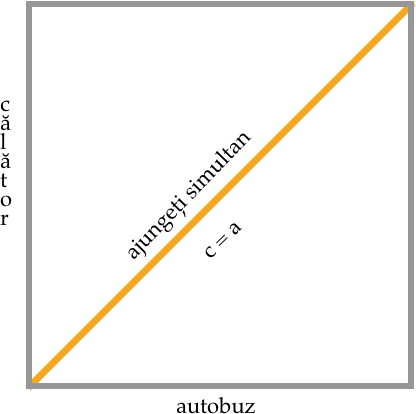
\includegraphics[scale=0.25]{imgs/c=a.png}
    \caption{$ c = a $}
  \end{subfigure} \quad
  \begin{subfigure}[b]{0.2\textwidth}
    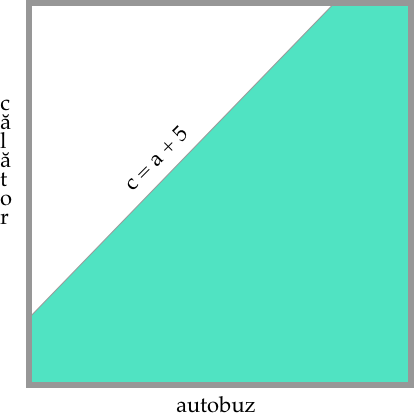
\includegraphics[scale=0.25]{imgs/c=a+5.png}
    \caption{$ c \leq a + 5 $}
  \end{subfigure} \quad
  \begin{subfigure}[b]{0.2\textwidth}
    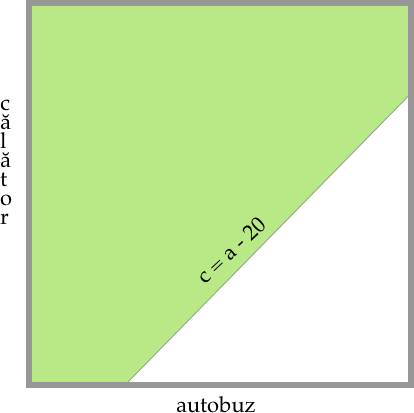
\includegraphics[scale=0.25]{imgs/c=b-20.png}
    \caption{$ c \leq a - 20 $}
  \end{subfigure} \quad
  \begin{subfigure}[b]{0.2\textwidth}
    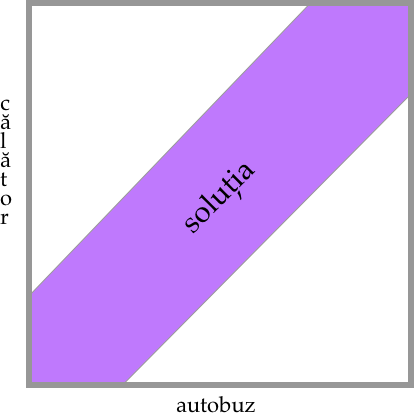
\includegraphics[scale=0.25]{imgs/solutie.png}
    \caption{Soluția}
  \end{subfigure}
  \caption{\emph{Problema autobuzului (cu așteptare)}}\label{fig:autobuz}
\end{figure}


\vspace{0.3cm}

15. Trei persoane aleg la întîmplare un număr real între 0 și 1. Care este probabilitatea
ca suma pătratelor numerelor alese de ei să nu depășească 1?

\emph{Soluție:} Pentru a modela problema geometric, e clar că o putem gîndi ca pe
alegerea unui punct din cubul unitate, $ (x, y, z) \in [0, 1]^3 $. Cazurile posibile sînt,
atunci, date de volumul cubului, care este 1.

Pentru cazurile favorabile, avem nevoie de $ x^2 + y^2 + z^2 \leq 1 $, care este sfera
unitate. Dar, cum ne interesează doar alegerile de numere pozitive, i.e.\ partea din
sferă care se găsește în interiorul cubului, adică $ \dfrac{1}{8} $ din ea.

Avem, deci:
\[
  P = \frac{ \frac{1}{8} \cdot \frac{4 \pi \cdot 1^3}{3}}{1} \simeq 52\%.
\]


\vspace{0.3cm}

Mult mai multe exemple sofisticate de probabilități geometrice se pot găsi la
\href{http://mathworld.wolfram.com/GeometricProbability.html}{Wolfram MathWorld}.


%%% Local Variables:
%%% mode: latex
%%% TeX-master: "../m3-19-20"
%%% End:
